\begin{figure}[H]
    \centering
    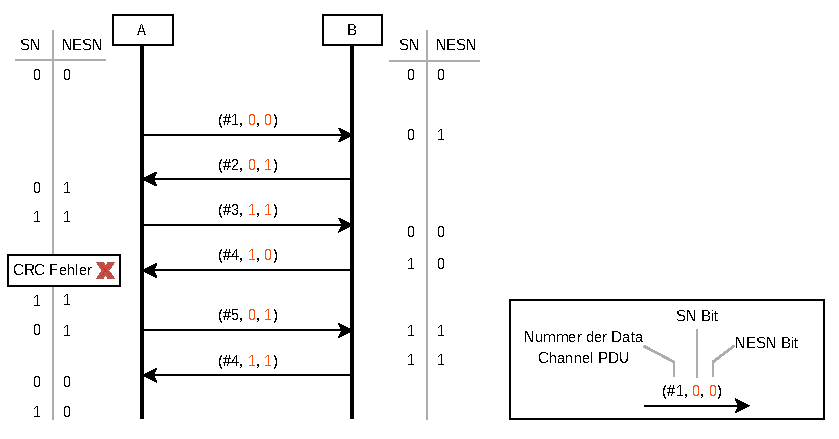
\includegraphics[width=0.9\textwidth]{graphics/nesn_sn_bsp.pdf}
    \caption[Beispiel für SN/NESN]{Beispiel für SN/NESN}
    \label{fig: anhang nesn sn}
\end{figure}
Gerät A und B verfügen jeweils über eigene Werte für SN/NESN und setzten diese jeweils auf 0 zu Beginn der Verbindung. Nun senden A und B gegenseitig Data Channel PDUs und nutzen folgenden Algorithmus für die SN/NESN. Die SN/NESN einer Data Channel PDU werden zur SN Bit bzw. NESN Bit genannt. Bei dem erstmaligen Empfang von Data Channel PDU \#4 gibt der CRC einen Fehler aus, also wurde das Paket nicht korrekt übertragen. 
\\\\
Algorithmus zum Setzen der SN/NESN \cite{BtSpec4.0_2239-2241} (bezieht sich immer nur auf das ausführende Gerät):
\\\\
Sei "`neue Data Channel PDU"' eine Data Channel PDU, die erstmalig gesendet wird (also keine erneute Sendung einer bereits gesendeten Data Channel PDU).\\
Sei "`alte Data Channel PDU"' eine Data Channel PDU, die bereits von dem Gerät gesendet bzw. empfangen wurde.\\
Sei "`letzte Data Channel PDU"' eine Data Channel PDU, die das Gerät zuletzt gesendet hat.
\begin{itemize}
    \item Senden einer Data Channel PDU:
    \begin{enumerate}
        \item Setze NESN Bit auf NESN. Falls Data Channel PDU eine neue Data Channel PDU ist, setze SN Bit auf SN
    \end{enumerate}
    \item Empfangen einer Data Channel PDU:
    \begin{enumerate}
        \item Ist SN Bit gleich NESN, dann wurde eine neue Data Channel PDU empfangen und NESN wird inkrementiert. Anderenfalls ist SN Bit ungleich NESN, also wurde eine alte Data Channel PDU empfangen, die ignoriert wird.
        \item Ist NESN Bit ungleich SN, dann wurde die letzte Data Channel PDU vom gegenüber bestätigt (ACK) und es wird SN inkrementiert. Anderenfalls ist NESN Bit gleich SN, also wurde die letzte Data Channel PDU nicht bestätigt (NAK) und muss erneut gesendet werden. Dabei muss SN Bit den Wert des SN Bit der letzten Data Channel PDU (also die zuletzt vom Gerät gesendet wurde) annehmen.
    \end{enumerate}
\end{itemize}
% - senden neuer Daten: SN bit auf SN setzen
% - senden Daten: NESN bit auf NESN setzen

% - empfangen Daten:
% SN bit ==  NESN, dann wurden neue Daten empfangen, NESN ++
% SN bit != NESN, dann wurden alte Daten empfangen
% NESN bit != SN, dann zuletzt gesendete Daten wurden ack., SN++
% NESN bit == SN, dann zuletzt gesendete Daten nak, diese erneut senden
% und dabei SN bit auf den Wert der Data Channel PDU
% setzen, die nicht empfangen wurde